\documentclass{article}
\usepackage[utf8]{inputenc}
\usepackage{hyperref,ragged2e,amsmath,multicol,gensymb,setspace,
fancyhdr,amsfonts,tikz,pgfplots,nccmath,enumerate,verbatim}
\usepackage[a4paper, width=216mm, height=297mm, margin=3cm]{geometry}
\usepgfplotslibrary{polar,fillbetween}
\usepgflibrary{shapes.geometric}
\usetikzlibrary{calc,patterns,arrows}
\newcommand\mylog[1]{\mathop{{}^{#1}\mathrm{log}}}
\pgfplotsset{compat=1.15}
\pgfplotsset{my style/.append style={axis x line=middle, axis y line=
middle, xlabel={$x$}, ylabel={$y$}, axis equal }}
\usepackage{etoolbox}
\newcommand{\zerodisplayskips}{%
  \setlength{\abovedisplayskip}{0pt}%
  \setlength{\belowdisplayskip}{0pt}%
  \setlength{\abovedisplayshortskip}{0pt}%
  \setlength{\belowdisplayshortskip}{0pt}}
\pagestyle{fancy}
\fancyhf{}
\lhead{Halaman \thepage}
\rhead{Persamaan Parametrik dan Koordinat Kutub   \\ (\href{https://twitter.com/ahmadzakiyudin_/}{@ahmadzakiyudin\_}) }
\hypersetup{
    colorlinks=true,
    linkcolor=blue,
    filecolor=blue,      
    urlcolor=blue,
}
\setlength{\columnsep}{0.8cm}
\begin{document}
\setstretch{1.3}
\section{Persamaan Parametrik}
Persamaan kurva yang titik-titiknya bergantung pada suatu parameter. Biasanya dituliskan
$$ x=x(t) \qquad y=y(t) \qquad (a\leq t\leq b)$$
Orientasi kurva parametrik merupakan arah pertambahan parameter.
Kurva parametrik dapat digambarkan dengan mengeliminasi parameter, tetapi menghilangkan informasi orientasi.
\section{Turunan Persamaan Parametrik}
Jika $x(t)$ dan $y(t)$ mempunyai turunan pertama terhadap $t$ yang kontinu dan $\dfrac{dx}{dt}\neq 0$, maka
$$ \dfrac{dy}{dx} = \dfrac{dy}{dt}\dfrac{dt}{dx} = \dfrac{\frac{dy}{dt}}{\frac{dx}{dt}} $$
Turunan keduanya sebagai berikut
$$ \dfrac{d^2y}{dx^2} = \dfrac{dy'}{dx} = \dfrac{\frac{d}{dt}\left(\frac{dy}{dx}\right)}{\frac{dx}{dt}} $$
Kurva parametrik memiliki garis singgung vertikal jika $\dfrac{dx}{dt}=0$ dan $\dfrac{dy}{dt}\neq 0$. Sedangkan jika $\dfrac{dx}{dt}\neq 0$ dan $\dfrac{dy}{dt}=0$, maka kurvanya memiliki garis singgung horizontal.
\section{Panjang Busur Kurva Parametrik}
Jika persamaan parametrik 
$$ x=x(t),\qquad y=y(t)\qquad (a\leq t\leq b) $$
ditelusuri tepat sekali saat $t$ bertambah dari $a$ ke $b$ dan $\dfrac{dx}{dt},\dfrac{dy}{dt}$ fungsi kontinu untuk $a\leq t\leq b$, maka panjang busur kurvanya adalah 
$$ S=\int_a^b \sqrt{\left(\dfrac{dx}{dt}\right)^2+\left(\dfrac{dy}{dt}\right)^2} \, dt $$
\section{Luas Permukaan Kurva Parametrik}
Luas permukaan kurva yang diputar terhadap sumbu$-x$
$$ S=\int_a^b 2\pi y(t)\sqrt{\left(\dfrac{dx}{dt}\right)^2+\left(\dfrac{dy}{dt}\right)^2} \, dt $$
Luas permukaan kurva yang diputar terhadap sumbu$-y$
$$ S=\int_a^b 2\pi x(t)\sqrt{\left(\dfrac{dx}{dt}\right)^2+\left(\dfrac{dy}{dt}\right)^2} \, dt $$
\section{Koordinat Kutub dan Koordinat Siku-Siku}
Titik $P(x,y)$ pada koordinat siku-siku memiliki koordinat $P(r,\theta)$ pada koordinat kutub dengan hubungan
$$ x=r\cos \theta \qquad y=r\sin\theta $$
dan 
$$ r^2=x^2+y^2\qquad \tan \theta =\dfrac{y}{x} $$
\section{Grafik dalam Koordinat Kutub}
Lingkaran yang berpusat di $(0,0)$ dan berjari-jari $a$ memiliki persamaan
$$ r = a $$
Lingkaran yang berpusat di sumbu$-x$ dan melewati titik $(0,0)$ serta berjari-jari $a$ memiliki persamaan
$$ r=2a\cos\theta \qquad \text{atau} \qquad r=-2a\cos\theta $$
Lingkaran yang berpusat di sumbu$-y$ dan melewati titik $(0,0)$ serta berjari-jari $a$ memiliki persamaan
$$ r=2a\sin\theta \qquad \text{atau} \qquad r=-2a\sin\theta $$
Kardioida dan limacons memiliki persamaan sebagai berikut 
$$ r=a\pm b\cos\theta \qquad\text{atau}\qquad r=a\pm b \sin\theta $$
dengan $a>0,b>0$\\
Jika $a<b$, maka terbentuk limacons berikut
\begin{center}
	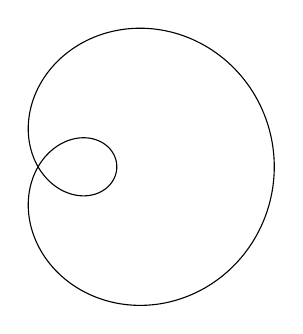
\begin{tikzpicture}
\begin{axis}[
x= 1 cm, y=1 cm,
 hide axis,
  xmin=-1,xmax=4,ymin=-2,ymax=2,
  xtick={0},
  ytick={0}]
\addplot[domain=0:360,samples=300,data cs=polar] (x,{1 + 2*cos(x)});
\end{axis}
\end{tikzpicture}
	\end{center}
Jika $a=b$, maka terbentuk kardioida berikut
\begin{center}
	\begin{tikzpicture}
\begin{axis}[
x= 1.5 cm, y=1.5 cm,
 hide axis,
  xmin=-1,xmax=4,ymin=-2,ymax=2,
  xtick={0},
  ytick={0}]
\addplot[domain=0:360,samples=300,data cs=polar] (x,{1 + cos(x)});
\end{axis}
\end{tikzpicture}
	\end{center}
Jika $b<a<2b$, maka terbentuk limacons cekung berikut
\begin{center}
	\begin{tikzpicture}
\begin{axis}[
x= 1.2 cm, y=1.2 cm,
 hide axis,
  xmin=-1,xmax=4,ymin=-2,ymax=2,
  xtick={0},
  ytick={0}]
\addplot[domain=0:360,samples=300,data cs=polar] (x,{1.2 + cos(x)});
\end{axis}
\end{tikzpicture}
	\end{center}
Jika $a\geq 2b$, maka terbentuk limacons cembung berikut
\begin{center}
	\begin{tikzpicture}
\begin{axis}[
x= 1 cm, y=1 cm,
 hide axis,
  xmin=-1,xmax=4,ymin=-2,ymax=2,
  xtick={0},
  ytick={0}]
\addplot[domain=0:360,samples=300,data cs=polar] (x,{1.6 + 0.8*cos(x)});
\end{axis}
\end{tikzpicture}
	\end{center} 
Lemniscate memiliki persamaan 
$$ r^2=\pm a^2\cos 2\theta \qquad \text{atau}\qquad r^2=\pm a^2\sin 2\theta $$
merupakan kurva yang berbentuk baling-baling sebagai berikut 
\begin{center}
	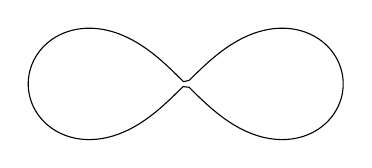
\begin{tikzpicture}
\begin{axis}[
x= 1 cm, y=1 cm,
 hide axis,
  xmin=-4,xmax=4,ymin=-2,ymax=2,
  xtick={0},
  ytick={0}]
\addplot[domain=0:360,samples=10000,data cs=polar] (x,2*sqrt{cos(2*x)});
\end{axis}
\end{tikzpicture}
	\end{center}
Posisi relatif ke sumbu kutub bergantung pada tanda di depan $a^2$ dan apakah $\sin 2\theta$ atau $\cos 2\theta$ yang muncul dalam persamaan.\\
Spiral memiliki persamaan bentuk 
$$ r=a\theta \quad (\theta\leq 0) $$
dengan kurva berikut
\begin{center}
	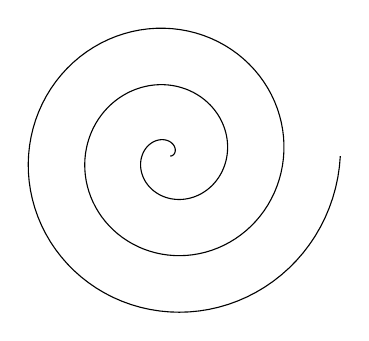
\begin{tikzpicture}
\begin{axis}[
x= 1 cm, y=1 cm,
 hide axis,
  xmin=-4,xmax=4,ymin=-2,ymax=2,
  xtick={0},
  ytick={0}]
\addplot[domain=0:360*3,samples=300,data cs=polar] (x,0.002*x);
\end{axis}
\end{tikzpicture}
	\end{center} 
Kurva rose yang memiliki persamaan 
$$ r=a\sin n\theta \qquad\text{atau}\qquad r=a\cos n\theta $$
berbentuk sebagai berikut 
\begin{center}
	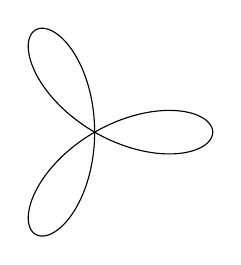
\begin{tikzpicture}
\begin{axis}[
x= 1.5 cm, y=1.5 cm,
 hide axis,
  xmin=-1,xmax=4,ymin=-2,ymax=2,
  xtick={0},
  ytick={0}]
\addplot[domain=0:360,samples=300,data cs=polar] (x,{cos(3*x)});
\end{axis}
\end{tikzpicture}
	\end{center}
Kurva ini memiliki $n$ daun jika $n$ ganjil dan $2n$ daun jika $n$ genap
\section{Luas dalam Koordinat Kutub}
Jika $r=f(\theta)$ kontinu dan tak negatif untuk $\alpha \leq \theta\leq \beta$ dan $0\leq \beta-\alpha\leq 2\pi$, maka luas kurvanya 
$$ A=\int_\alpha^\beta \dfrac{1}{2}[f(\theta)]^2\, d\theta = \int_\alpha^\beta \dfrac{1}{2} r^2 d\theta $$
\section{Volume Benda Putar dalam Koordinat Kutub}
Volume benda putar yang diputar terhadap sumbu$-x$ dan dibatasi oleh $\theta_1=\alpha$ dan $\theta_2=\beta$ adalah 
$$ V=\int_\alpha^\beta \dfrac{2}{3}\pi r^3\sin\theta \, d\theta $$
Volume benda putar yang diputar terhadap sumbu$-y$ dan dibatasi oleh $\theta_1=\alpha$ dan $\theta_2=\beta$ adalah 
$$ V=\int_\alpha^\beta \dfrac{2}{3}\pi r^3\cos\theta \, d\theta $$
\section{Turunan Persamaan Kurva Kutub}
Jika $r=f(\theta)$, maka 
$$ \dfrac{dy}{dx} = \dfrac{\frac{dy}{d\theta}}{\frac{dx}{d\theta}} = \dfrac{r\cos\theta +\sin\theta \frac{dr}{d\theta}}{-r\sin\theta+\cos\theta \frac{dr}{d\theta}} $$
\section{Panjang Busur Kurva Kutub}
Jika kurva $r=f(\theta)$ ditelusuri tepat sekali untuk $\theta$ bertambah dari $\alpha$ ke $\beta$ dan $\dfrac{dr}{d\theta}$ kontinu untuk $\alpha\leq \theta\leq \beta$, maka panjang busur kurva
$$ S=\int_\alpha^\beta \sqrt{r^2+\left(\dfrac{dr}{d\theta}\right)^2}\, d\theta $$
\section{Latihan Soal}
\begin{enumerate}
	\item \begin{enumerate}
		\item Buatlah sketsa kurva dari persamaan parametrik 
		$$ x=1+\cos t, ~~ y=3-\sin t, ~~ 0\leq t\leq 2\pi $$
		\item Dapatkan panjang busur dari kurva tersebut.
		\item Dapatkan semua nilai parameter $t$ yang menyebabkan kurva tersebut mempunyai garis singgung vertikal 
	\end{enumerate}
	\textbf{Penyelesaian:}
	\begin{enumerate}
		\item Tinjau bahwa $\cos t=x-1$ dan $\sin t=3-y$ sehingga $\cos^2 t+\sin^2 t =1=(x-1)^2+(3-y)^2$ \\Diperoleh persamaan lingkaran yang berpusat di $(1,3)$ dan berjari-jari 1. Karena $0\leq t\leq 2\pi$, maka kurvanya merupakan satu lingkaran penuh sebagai berikut
		\begin{center}
	\begin{tikzpicture}
\begin{axis}[
x= 1 cm, y=1 cm,
 axis lines=middle,
  xmin=-0.5,xmax=3,ymin=-0.5,ymax=4.2,
  xtick distance=1,
  ytick distance=1,
  xlabel=$x$,
  ylabel=$y$]
\draw (1,3) circle[radius=1 cm];
\end{axis}
\end{tikzpicture}
	\end{center}
	\item Karena kurvanya merupakan satu lingkaran penuh dengan jari-jari 1, maka panjang busurnya adalah keliling lingkaran yaitu $2\pi r=2\pi$\\
	Dapat dihitung pula dengan rumus panjang busur untuk kurva parametrik, yaitu 
	$$ S=\int_a^b \sqrt{\left(\dfrac{dx}{dt}\right)^2+\left(\dfrac{dy}{dt}\right)^2}\, dt $$ 
	Tinjau 
	$$ \dfrac{dx}{dt} = -\sin t \text{   dan   } \dfrac{dy}{dt}=-\cos t $$
	serta $a=0$ dan $b=2\pi$ sehingga 
	\begin{align*}
	S &= \int_0^{2\pi}\sqrt{(-\sin t)^2+(-\cos t)^2}\, dt\\
	&= \int_0^{2\pi}\, dt\\
	&= t\big|_0^{2\pi}\\
	&= 2\pi 
	\end{align*}
	\item Kurva tersebut mempunyai garis singgung vertikal jika $\dfrac{dx}{dt}=0$ dan $\dfrac{dy}{dt}\neq 0$, yaitu saat $t=0$, $t=\pi$, dan $t=2\pi$
	\end{enumerate}
	\item Dapatkan panjang busur dari kurva $r=a\cos \theta+b\sin\theta$. (Berikan gambar sketsa kurvanya).\\
	Perhatikan: bilangan $b$ dan $a$ dalam soal ini adalah dua digit terakhir NRP anda. Misalkan NRP anda adalah 06111940000076 maka $b=7$ dan $a=6$, jika $a$ atau $b$ adalah 0 ganti dengan angka 10.\\
	\textbf{Penyelesaian:}\\
	Ingat rumus panjang busur untuk kurva kutub $r=f(\theta)$ jika kurvanya ditelusuri keseluruhan satu kali untuk $\theta$ bergerak dari $\theta=\alpha$ ke $\theta=\beta$ adalah 
	$$ \int_{\alpha}^{\beta}\sqrt{r^2+\left(\dfrac{dr}{d\theta}\right)^2} \, d\theta $$
	Perhatikan bahwa
	\begin{align*}
	r^2 + \left(\dfrac{dr}{d\theta}\right)^2 &= ( a\cos \theta+b\sin\theta)^2+(-a\sin \theta+b\cos\theta)^2\\
	&= a^2\cos^2 \theta+2ab\cos\theta\sin\theta+b^2\sin^2\theta+a^2\sin^2\theta-2ab\sin\theta\cos\theta+b^2\cos^2\theta\\
	&= a^2+b^2
	\end{align*}
	Tinjau bahwa kurva tersebut ditelusuri keseluruhan satu kali untuk $\theta$ bergerak dari $\theta=0$ ke $\theta=\pi$, karena titik $(a,0)$ dan titik $(-a,\pi)$ merupakan titik yang sama dalam koordinat kutub. Jadi diperoleh 
	\begin{align*}
	S &= \int_0^\pi \sqrt{a^2+b^2}\, d\theta\\
	&= \theta\sqrt{a^2+b^2}\big|^\pi_0\\
	&= \pi\sqrt{a^2+b^2} 
	\end{align*}
	Untuk menggambar kurvanya, ingat bahwa $\dfrac{x}{r}=\cos \theta$ dan $\dfrac{y}{r}=\sin \theta$, serta $x^2+y^2=r^2$ sehingga
	\begin{align*}
	r &= a\cos\theta+b\sin\theta\\
	r &= \dfrac{ax}{r}+\dfrac{by}{r}\\
	r^2 &= ax+by\\
	x^2+y^2-ax-by &= 0 \\
	\left(x-\frac{a}{2}\right)^2+\left(y-\frac{b}{2}\right)^2 -\dfrac{a^2}{4}-\dfrac{b^2}{4} &= 0\\
	\left(x-\frac{a}{2}\right)^2+\left(y-\frac{b}{2}\right)^2 &= \dfrac{a^2+b^2}{4}
	\end{align*}
	Jadi kurvanya merupakan lingkaran yang berpusat di $\left(\frac{a}{2},\frac{b}{2}\right)$ dan berjari-jari $\frac{\sqrt{a^2+b^2}}{2}$\\
	Jika $a=6$ dan $b=7$, maka lingkarannya berpusat di $(3,3.5)$ dan berjari-jari $\frac{\sqrt{85}}{2}$, serta memotong titik $(0,0),(6,0),$ dan $(0,7)$ sebagai berikut
	\begin{center}
	\begin{tikzpicture}
\begin{axis}[
x= 0.7 cm, y=0.7 cm,
 axis lines=middle,
  xmin=-1.8,xmax=8,ymin=-1.5,ymax=9,
  xtick={0,3,6},
  ytick={0,7},
  xlabel=$x$,
  ylabel=$y$]
\draw (3,3.5) circle[radius=0.7*4.60977 cm];
\end{axis}
\end{tikzpicture}
	\end{center}
	Cara lain untuk mendapatkan panjang busurnya adalah menghitung keliling lingkaran tersebut yang berjari-jari $r=\frac{\sqrt{a^2+b^2}}{2}$, yaitu $S=2\pi r=2\pi\frac{\sqrt{a^2+b^2}}{2}=\pi\sqrt{a^2+b^2}$
	\item Diberikan partikel bergerak sepanjang kurva $\begin{cases}x=1-t\\ y=\sqrt{8+2t-t^2}\end{cases}$ dengan $-2\leq t\leq 1$
	\begin{enumerate}
		\item Nyatakan dalam persamaan kutub $r=f(\theta)$ dengan lintasan $\theta$
		\item Tentukan panjang lintasan kurva tersebut
		\item Sketsa persamaan kurva tersebut dan arah lintasannya 
	\end{enumerate}
	\textbf{Penyelesaian:}
	\begin{enumerate}
		\item Perhatikan bahwa $t=1-x$ sehingga
		\begin{align*}
		y&=\sqrt{8+2(1-x)-(1-x)^2}\\
		&=\sqrt{8+2-2x-1+2x-x^2}\\
		&= \sqrt{9-x^2}
		\end{align*}
		Ingat bahwa $y=r\sin\theta$ dan $x=r\cos\theta$ sehingga
		\begin{align*}
		r\sin\theta &=\sqrt{9-r^2\cos^2\theta}\\
		r^2\sin^2\theta &= 9-r^2\cos^2\theta\\
		r^2 &= 9
		\end{align*}
		Dapat diambil $r=f(\theta)=3$. Untuk $t=-2$, maka $x=r\cos\theta=3$ sehingga $\theta=0$, dan untuk $t=1$, maka $x=r\cos\theta=0$ sehingga $\theta=\dfrac{\pi}{2}$. Jadi $r=f(\theta)=3$ dengan $0\leq \theta\leq\dfrac{\pi}{2}$
		\item Tinjau bahwa $r=3$ dengan $0\leq \theta\leq \dfrac{\pi}{2}$ merupakan seperempat lingkaran dengan jari-jari $r=3$ di kuadran pertama, sehingga panjang lintasan kurva tersebut merupakan seperempat keliling lingkaran yaitu $\dfrac{1}{4}\cdot 2\pi r=\dfrac{3}{2}\pi$
		\item Dari jawaban (b) sudah diperoleh bentuk kurvanya.\\
		Sedangkan untuk arah lintasannya, tinjau bahwa $x$ berkurang dan $y$ bertambah ketika $t$ bergerak dari $-2$ ke 1, sehingga arahnya berlawanan arah jarum jam. Berikut sketsanya
		\begin{center}
	\begin{tikzpicture}
\begin{axis}[
x= 1.4 cm, y=1.4 cm,
 axis lines=middle,
  xmin=-0.5,xmax=3.5,ymin=-0.5,ymax=3.5,
  xtick distance=1,
  ytick distance=1,
  xlabel=$x$,
  ylabel=$y$]
\addplot[domain=0:90,samples=300,data cs=polar] (x,{3});
\end{axis}
\end{tikzpicture}
	\end{center}
	\end{enumerate}
	\item Gambarkan dan dapatkan luas irisan dari $r=\sin 2\theta$ dan $r=\cos \theta$\\
	\textbf{Penyelesaian:}\\
	Perhatikan bahwa $r_1=\sin 2\theta$ merupakan kurva rose dengan $n$ genap sehingga memiliki 4 daun sebagai berikut
	\begin{center}
	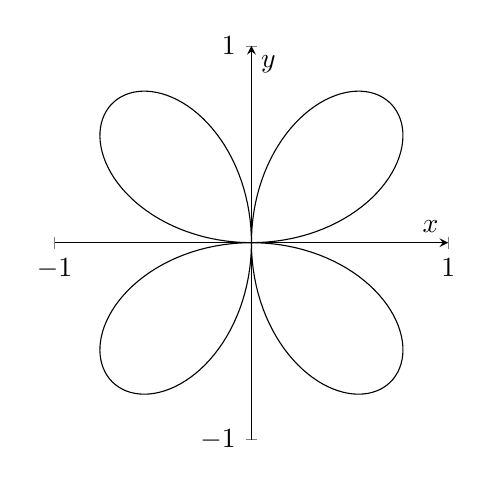
\begin{tikzpicture}
\begin{axis}[
x= 2.5 cm, y=2.5 cm,
 axis lines=middle,
  xmin=-1,xmax=1,ymin=-1,ymax=1,
  xtick distance=1,
  ytick distance=1,
  xlabel=$x$,
  ylabel=$y$]
\addplot[domain=0:360,samples=300,data cs=polar] (x,{sin(2*x)});
\end{axis}
\end{tikzpicture}
	\end{center}
	Sedangkan $r=\cos \theta$ merupakan lingkaran yang berpusat di $(0.5,0)$ dan berjari-jari $0.5$ sebagai berikut
	\begin{center}
	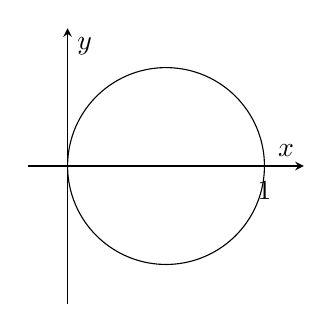
\begin{tikzpicture}
\begin{axis}[
x= 2.5 cm, y=2.5 cm,
 axis lines=middle,
  xmin=-0.2,xmax=1.2,ymin=-0.7,ymax=0.7,
  xtick distance=1,
  ytick distance=1,
  xlabel=$x$,
  ylabel=$y$]
\addplot[domain=0:360,samples=5000,data cs=polar] (x,{cos(x)});
\end{axis}
\end{tikzpicture}
	\end{center}
	Dapat diperoleh irisannya sebagai berikut 
	\begin{center}
	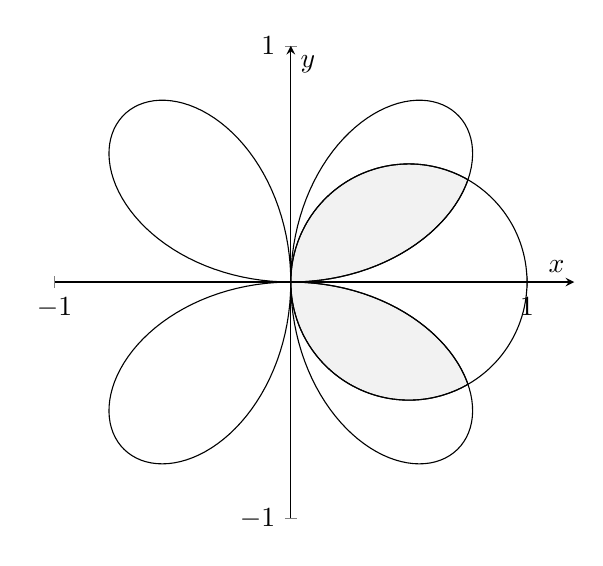
\begin{tikzpicture}
\begin{axis}[
x= 3 cm, y=3 cm,
 axis lines=middle,
  xmin=-1,xmax=1.2,ymin=-1,ymax=1,
  xtick distance=1,
  ytick distance=1,
  xlabel=$x$,
  ylabel=$y$]
\addplot[domain=0:360,samples=5000,data cs=polar] (x,{cos(x)});
\addplot[domain=0:360,samples=300,data cs=polar] (x,{sin(2*x)});
\addplot[domain=30:90,name path = B,samples=300,data cs=polar] (x,{cos(x)});
\addplot[domain=0:30,name path = A,samples=300,data cs=polar] (x,{sin(2*x)});
\addplot[domain=270:330,name path = C,samples=300,data cs=polar] (x,{cos(x)});
\addplot[domain=150:180,name path = D,samples=300,data cs=polar] (x,{sin(2*x)});
\addplot[gray,opacity=0.1] fill between[of=B and A];
\addplot[gray,opacity=0.1] fill between[of=C and D];
\end{axis}
\end{tikzpicture}
	\end{center}
	Perhatikan bahwa kurvanya simetris sehingga cukup hitung luas pada kuadran I kemudian kalikan 2. Tinjau titik perpotongan pada kuadran I adalah 
	\begin{align*}
	r_1 &= r_2\\
	\sin 2\theta &=\cos \theta\\
	2\sin \theta \cos \theta -\cos\theta &= 0\\
	\cos\theta(2\sin\theta -1) &=0
	\end{align*}
	Diperoleh perpotongannya ketika $\cos\theta=0$ yaitu $\theta_2=\dfrac{\pi}{2}$ untuk $r_2=\cos \theta$ dan $\theta_1=0$ untuk $r_1=\sin 2\theta$. Ketika $\sin\theta = \dfrac{1}{2}$, maka $\theta_1=\theta_2=\dfrac{\pi}{6}$. Jadi, luas irisan kurva pada kuadran I dapat dirumuskan
	\begin{align*}
	L &= \int_0^\frac{\pi}{6} \dfrac{1}{2} r_1^2 \, d\theta + \int_\frac{\pi}{6}^\frac{\pi}{2}\dfrac{1}{2}r_2^2 \, d\theta\\
	&= \dfrac{1}{2} \int_0^\frac{\pi}{6} \sin^2 2\theta \, d\theta + \dfrac{1}{2} \int_\frac{\pi}{6}^\frac{\pi}{2} \cos^2\theta \, d\theta \\
	&= \dfrac{1}{2} \int_0^\frac{\pi}{6} \dfrac{1-\cos 4\theta}{2}\, d\theta + \dfrac{1}{2} \int_\frac{\pi}{6}^\frac{\pi}{2} \dfrac{1+\cos 2\theta}{2}\, d\theta \\
	&= \dfrac{1}{4}\left[\theta -\dfrac{\sin 4\theta}{4}\right]_0^\frac{\pi}{6} + \dfrac{1}{4}\left[\theta+\dfrac{\sin 2\theta}{2}\right]_\frac{\pi}{6}^\frac{\pi}{2}\\
	&= \dfrac{1}{4}\left[\dfrac{\pi}{6}-\dfrac{1}{8}\sqrt{3}+\dfrac{\pi}{2}+0-\dfrac{\pi}{6}-\dfrac{1}{4}\sqrt{3}\right]\\
	&= \dfrac{\pi}{8}-\dfrac{3}{32}\sqrt{3}
	\end{align*}
	Jadi luas total irisan adalah $2L=\dfrac{\pi}{4}-\dfrac{3}{16}\sqrt{3}$
	\item Dapatkan kemiringan garis singgung pada kurva $r=3\sin 3\theta$ di $\theta=\dfrac{\pi}{4}$\\
	\textbf{Penyelesaian:}\\
	Ingat bahwa kemiringan garis singgung kurva di suatu titik merupakan turunan persamaan kurva tersebut di titik itu, dan turunan persamaan kurva kutub adalah
	$$ \dfrac{dy}{dx} = \dfrac{\frac{dy}{d\theta}}{\frac{dx}{d\theta}} = \dfrac{r\cos\theta +\sin\theta \frac{dr}{d\theta}}{-r\sin\theta+\cos\theta \frac{dr}{d\theta}} $$
	sehingga diperoleh 
	\begin{align*}
	\dfrac{dy}{dx} &= \dfrac{3\sin 3\theta \cos \theta+\sin \theta (9\cos 3\theta)}{-3\sin 3\theta\sin\theta +\cos\theta (9\cos 3\theta)}
	\end{align*}
	Untuk $\theta=\dfrac{\pi}{4}$, maka 
	\begin{align*}
	\dfrac{dy}{dx} &= \dfrac{3\left( \frac{1}{2}\sqrt{2}\right)\left( \frac{1}{2}\sqrt{2}\right)+9\left( \frac{1}{2}\sqrt{2}\right) \left(-\frac{1}{2}\sqrt{2}\right)}{-3\left(\frac{1}{2}\sqrt{2}\right)\left(\frac{1}{2}\sqrt{2}\right)+9\left(\frac{1}{2}\sqrt{2}\right)\left(-\frac{1}{2}\sqrt{2}\right)}\\
	&= \dfrac{\frac{3}{2}-\frac{9}{2}}{-\frac{3}{2}-\frac{9}{2}}\\
	&= \dfrac{-3}{-6} = \dfrac{1}{2}
	\end{align*}
	Jadi kemiringan garis singgung pada kurva $r=3\sin 3\theta$ di $\theta=\dfrac{\pi}{4}$ adalah $\dfrac{1}{2}$
\end{enumerate}
\end{document}
